\begin{figure}[H]
  \centering
  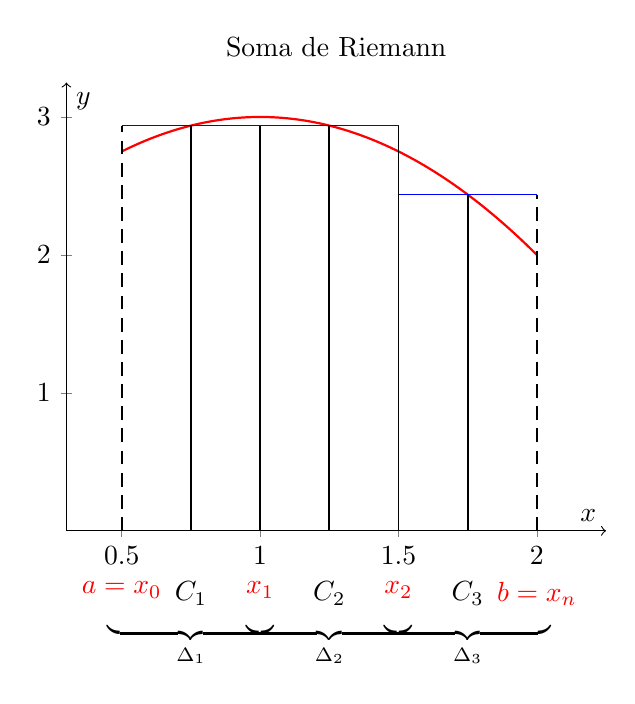
\begin{tikzpicture}
    \begin{axis}[
      xmin=0.3, xmax=2.25,
      ymin=0, ymax=3.25,
      axis x line=middle,
      axis y line=middle,
      axis line style={->},
      xlabel={$x$},
      ylabel={$y$},
      title={Soma de Riemann},
      clip=false,
      %xticklabels={}
    ]
      % curva
      \addplot[red, thick, domain=0.5:2, samples=200] {2*x - x^2 + 2};

      % retângulos da soma
      \draw[dash pattern=on 5pt off 3pt, line width=0.6pt]  (axis cs:0.5,0) -- (axis cs:0.5,{2*0.75 - 0.75^2 + 2});
      \draw[line width=0.6pt] (axis cs:0.75,0) -- (axis cs:0.75,{2*0.75 - 0.75^2 + 2});
      \draw[line width=0.6pt] (axis cs:1,0)    -- (axis cs:1,{2*0.75 - 0.75^2 + 2});
      \draw[line width=0.6pt] (axis cs:1.25,0) -- (axis cs:1.25,{2*1.25 - 1.25^2 + 2});
      \draw[line width=0.6pt] (axis cs:1.5,0)  -- (axis cs:1.5,{2*1.25 - 1.25^2 + 2});
      \draw[line width=0.6pt] (axis cs:1.75,0) -- (axis cs:1.75,{2*1.75 - 1.75^2 + 2});
      \draw[dash pattern=on 5pt off 3pt, line width=0.6pt]  (axis cs:2,0) -- (axis cs:2,{2*1.75- 1.75^2 + 2});
      % linhas de fechamento do topo
      \draw[blue, line width=0.6] (axis cs:0.5,2*0.75-0.75^2+2) -- (1,2*0.75-0.75^2+2);
      \draw[blue, line width=0.6] (axis cs:1,2*1.25-1.25^2+2) -- (1.5,2*1.25-1.25^2+2);
      \draw[blue, line width=0.6] (axis cs:1.5,2*1.75-1.75^2+2) -- (2,2*1.75-1.75^2+2);

      % marcas no eixo x
      \node[below, text=red] at (axis cs:0.5,-0.3) {$a=x_0$};
      \node[below, text=black] at (axis cs:0.75,-0.3) {$C_1$};
      \node[below, text=black] at (axis cs:0.75,-0.6) {$\underbrace{\hspace{6em}}_{\Delta_1}$};
      \node[below, text=red] at (axis cs:1,-0.3) {$x_1$};
      \node[below, text=black] at (axis cs:1.25,-0.3) {$C_2$};
      \node[below, text=black] at (axis cs:1.25,-0.6) {$\underbrace{\hspace{6em}}_{\Delta_2}$};
      \node[below, text=red] at (axis cs:1.5,-0.3) {$x_2$};
      \node[below, text=black] at (axis cs:1.75,-0.3) {$C_3$};
      \node[below, text=black] at (axis cs:1.75,-0.6) {$\underbrace{\hspace{6em}}_{\Delta_3}$};
      \node[below, text=red] at (axis cs:2,-0.3) {$b=x_n$};
          \end{axis}
  \end{tikzpicture}
  \caption{Aproximação da área sob $f(x)=2x-x^2+2$ por retângulos.}
\end{figure}